%\section{Appendix}
\section{Set-of-Records Cleaning Model}\label{set-of-r}
In paper, we formalized the analyst-specified data cleaning as follows.
We take the sample of the records $S_{dirty}$, and apply data cleaning $C(\cdot)$.
$C$ is applied to a record and produces the clean record:
\[
S_{clean} = \{C(r) : \forall r \in S_{dirty}\}
\]
The record-by-record cleaning model is a formalization of the costs of data cleaning where each record has the same cost to clean and this cost does not change throughout the entire cleaning session.
There are, however, some cases when cleaning the first record of a certain type of corruption is expensive but all subsequent records are cheaper.

\begin{example}\label{app-ex1}
In most spell checking systems, when a misspelling is identified, the system gives an option to fix all instances of that misspelling.
\end{example}

\begin{example}\label{app-ex2}
When an inconsistent value is identified all other records with the same inconsistency can be efficiently fixed.
\end{example}

This model of data cleaning can fit into our framework and we formalize it as the ``Set-of-Records" model as opposed to the ``Record-by-Record" model. 
In this model, the cleaning function $C(\cdot)$ is not restricted to updating only the records in the sample.
$C(\cdot)$ takes the entire dirty sample as an argument (that is the cleaning is a function of the sample), the dirty data, and updates the entire dirty data:
\[
R'_{dirty} = C(S_{dirty},R_{dirty})
\]
we require that for every record $s \in S_{dirty}$, that record is completely cleaned after applying $C(\cdot)$, giving us $S_{clean}$.
Records outside of $S_{dirty}$ may be cleaned on a subset of dirty attributes by $C(\cdot)$.
After each iteration, we re-run the detector, and move any $r \in R'_{dirty}$ that are clean to $R_{clean}$.
Such a model allows us to capture data cleaning operations such as in Example \ref{app-ex1} and Example \ref{app-ex2}.

\section{Stochastic Gradient Descent}\label{appsgd}

Stochastic Gradient Descent converges for a suitably chosen step size if the sample gradients are unbiased estimates of the full gradient. 
The first problem is to choose weights $\alpha$ and $\beta$ (to average already clean and newly cleaned data) such that the estimate of the gradient is unbiased. 
%SGD will converge when the estimate is unbiased and the step-size is chosen appropriately.
The batch $S_{dirty}$ is drawn only from $R_{dirty}$.
Since the sizes of $R_{dirty}$ and its complement are known, it follows that the gradient over the already clean data $g_C$ and the recently cleaned data $g_S$ can be combined as follows:
\[
g(\theta^{t}) = \frac{\mid R_{dirty} \mid \cdot g_S + \mid R_{clean} \mid \cdot g_C  }{\mid R \mid}
\]
Therefore,
\[
\alpha = \frac{\mid R_{clean} \mid}{\mid R \mid}, \beta = \frac{\mid R_{dirty} \mid}{\mid R \mid}
\]

\begin{lemma}
The gradient estimate $g(\theta)$ is unbiased if $g_S$ is an unbiased estimate of:
\[
\frac{1}{\mid R_{dirty} \mid} \sum g_i(\theta)
\]
\end{lemma}
\begin{proof}[Sketch]
\[
\mathbb{E}(\frac{1}{\mid R_{dirty} \mid} \sum g_i(\theta)) = \frac{1}{\mid R_{dirty} \mid} \cdot \mathbb{E}(\sum g_i(\theta)))
\]
By symmetry, 
\[
\mathbb{E}(\frac{1}{\mid R_{dirty} \mid} \sum g_i(\theta)) = g(\theta)
\]
\[
\mathbb{E}(\frac{1}{\mid R_{dirty} \mid} \sum g_i(\theta)) = \frac{\mid R_{dirty} \mid \cdot g_S + \mid R_{clean} \mid \cdot g_C  }{\mid R \mid}
\]
\end{proof}

The error bound discussed in Proposition 2 can be tightened for a class of models called strongly convex (see \cite{bertsekas2011incremental} for a defintion). 

\begin{proposition}
For a strongly convex loss, a batch size $b$, and $T$ iterations, the convergence rate is bounded by $O(\frac{\sigma^2}{bT})$. 
\end{proposition}

\section{Non-convex losses}\label{non-convex}
We acknowledge that there is an increasing popularity of non-convex losses in the Neural Network and Deep Learning literature. 
However, even for these losses, gradient descent techniques still apply. 
Instead of converging to a global optimum they converge to a locally optimal value. 
Likewise, \sys will converge to the closest locally optimal value to the dirty model. 
Because of this, it is harder to reason about the results.
Different initializations will lead to different local optima, and thus, introduces a complex dependence on the initialization with the dirty model.
This problem is not fundemental to \sys and any gradient technique suffers this challenge for general non-convex losses, and we hope to explore this more in the future.

\section{Importance Sampling}\label{impsample-deriv}
This lemma describes the optimal distribution over a set of scalars:
\begin{lemma}\label{impsample}
Given a set of real numbers $A = \{a_1,...,a_n\}$, let $\hat{A}$ be 
a sample with replacement of $A$ of size k.
If $\mu$ is the mean $\hat{A}$, the sampling distribution that minimizes
 the variance of $\mu$, i.e., the expected square error, is $p(a_i) \propto a_i$.
\end{lemma}
Lemma \ref{impsample} shows that when estimating a mean of numbers with sampling, the distribution with optimal variance is sampling proportionally to the values.

The variance of this estimate is given by:
\[
Var(\mu) = \mathbb{E}(\mu^2)-\mathbb{E}(\mu)^2
\] 
Since the estimate is unbiased, we can replace $\mathbb{E}(\mu)$ with the average of $A$:
\[
Var(\mu) = \mathbb{E}(\mu^2)-\bar{A}^2
\]
Since $\bar{A}$ is deterministic, we can remove that term during minimization.
Furthermore, we can write $\mathbb{E}(\mu^2)$ as:
\[
\mathbb{E}(\mu^2) = \frac{1}{n^2}\sum_i^n \frac{a_i^2}{p_i}
\]
Then, we can solve the following optimization problem (removing the proportionality of $\frac{1}{n^2}$) over the set of weights $P=\{p(a_i)\}$:
\[
\min_{P} \sum_i^N \frac{a_i^2}{p_i}
\]
\[
\text{subject to: } P > 0, \sum P = 1
\]
Applying Lagrange multipliers, an equivalent unconstrained optimization problem is:
\[
\min_{P > 0,\lambda > 0} \sum_i^N \frac{a_i^2}{p_i} + \lambda \cdot (\sum P - 1)
\]
If, we take the derivatives with respect to $p_i$ and set them equal to zero:
\[
-\frac{a_i^2}{2 \cdot p_i^2} + \lambda = 0
\]
If, we take the derivative with respect to $\lambda$ and set it equal to zero:
\[
\sum P - 1
\]
Solving the system of equations, we get:
\[
p_i = \frac{\mid a_i \mid }{\sum_i \mid a_i \mid}
\]

\section{Linearization}\label{apptaylor}
If $d$ is the dirty value and $c$ is the clean value, the Taylor series approximation for a function $f$ is given as follows:
\[
f(c) = f(d) + f'(d)\cdot(d-c) + ...
\]
Ignoring the higher order terms, the linear term $f'(d)\cdot(d-c)$ is a linear function in each feature and label.
We only have to know the change in each feature to estimate the change in value.
In our case the function $f$ is the gradient $\nabla\phi$.
So, the resulting linearization is:
\[
\nabla\phi(x^{(c)}_i,y^{(c)}_i,\theta) \approx \nabla\phi(x,y,\theta) + \frac{\partial}{\partial X}\nabla\phi(x,y,\theta)\cdot (x - x^{(c)}) \]
\[+ \frac{\partial}{\partial Y}\phi(x,y,\theta)\cdot (y - y^{(c)})
\]
When we take the expected value:
\[
\mathbb{E}(\nabla\phi(x_{clean},y_{clean},\theta)) \approx \nabla\phi(x,y,\theta) + \frac{\partial}{\partial X}\nabla\phi(x,y,\theta)\cdot \mathbb{E}(\Delta x) \]
\[+ \frac{\partial}{\partial Y}\nabla\phi(x,y,\theta)\cdot \mathbb{E}(\Delta y)
\]
It follows that:
\[
\approx \nabla\phi(x,y,\theta) + M_x \cdot \mathbb{E}(\Delta x) + M_y \cdot \mathbb{E}(\Delta y)
\]
where $M_x = \frac{\partial}{\partial X}\nabla\phi$ and $M_y = \frac{\partial}{\partial Y}\nabla\phi$.
Recall that the feature space is $d$ dimensional and label space is $l$ dimensional.
Then, $M_x$ is an $d \times d$ matrix, and $M_y$ is a $d \times l$ matrix.
Both of these matrices are computed for each record.
$\Delta x$ is a $d$ dimensional vector where each component represents a change in that feature and $\Delta y$ is an $l$ dimensional vector that represents the change in each of the labels. 

This linearization allows \sys to maintain per feature (or label) average changes and use these changes to center the optimal sampling distribution around the expected clean value.
To estimate $\mathbb{E}(\Delta x)$ and $\mathbb{E}(\Delta y)$, consider the following for a single feature $i$:
If we average all $j=\{1,...,K\}$ records cleaned that have an error for that feature, weighted by their sampling probability:
\[
\bar{\Delta}_{xi} = \frac{1}{NK}\sum_{j=1}^K (x^{(d)}[i]-x^{(c)}[i])\times \frac{1}{p(j)}
\]
Similarly, for a label $i$:
\[
\bar{\Delta}_{yi} = \frac{1}{NK}\sum_{j=1}^K (y^{(d)}[i]-y^{(c)}[i])\times \frac{1}{p(j)}
\]

Each $\bar{\Delta}_{xi}$ and $\bar{\Delta}_{yi}$ represents an average change in a single feature.
A single vector can represent the necessary changes to apply to a record $r$:
For a record $r$, the set of corrupted features is $f_r,l_r$.
Then, each record $r$ has a d-dimensional vector $\Delta_{rx}$ which is constructed as follows:
\[
 \Delta_{rx}[i] = \begin{cases} 0 & i \notin f_r \\ 
\bar{\Delta}_{xi} & i \in f_r
\end{cases} 
\]
Each record $r$ also has an l-dimensional vector $\Delta_{ry}$ which is constructed as follows:
\[
 \Delta_{rx}[i] = \begin{cases} 0 & i \notin l_r \\ 
\bar{\Delta}_{yi} & i \in l_r
\end{cases} 
\]
Finally, the result is: 
\[p_{r}\propto\|\nabla\phi(x,y,\theta^{(t)}) + M_x \cdot \Delta_{rx} +  M_y \cdot \Delta_{ry}\|
\]

\section{Example $M_x$, $M_y$}\label{example-deriv}
\noindent\textbf{Linear Regression: }
\[
\nabla\phi(x,y,\theta) = (\theta^Tx - y)x
\]
For a record, $r$, suppose we have a feature vector $x$.
If we take the partial derivatives with respect to x, $M_x$ is:
\[
M_x[i,i] = 2x[i] + \sum_{i \ne j} \theta[j]x[j] - y 
\]
\[
M_x[i,j] = \theta[j]x[i]
\]
Similarly $M_y$ is:
\[
M_y[i,1] = x[i] 
\]

\vspace{0.5em}

\noindent\textbf{Logistic Regression: } 
\[
\nabla\phi(x,y,\theta) = (h(\theta^Tx) - y)x
\]
where
\[
h(z) = \frac{1}{1+e^{-z}}
\]
we can rewrite this as:
\[
h_{\theta}(x) = \frac{1}{1+e^{\theta^Tx}}
\]
\[
\nabla\phi(x,y,\theta) = (h_{\theta}(x) - y)x
\]
In component form,
\[
g = \nabla\phi(x,y,\theta)
\]
\[
g[i] = h_{\theta}(x)\cdot x[i] - yx[i]
\]
Therefore,
\[
M_x[i,i] = h_{\theta}(x)\cdot(1- h_{\theta}(x))\cdot \theta[i] x[i] + h_{\theta}(x) - y
\]
\[
M_x[i,j] = h_{\theta}(x)\cdot(1- h_{\theta}(x))\cdot \theta[j] x[i] + h_{\theta}(x)
\]
\[
M_y[i,1] = x[i] 
\]

\noindent\textbf{SVM: } 
\[
\nabla\phi(x,y,\theta) =
\begin{cases}      
-y\cdot\boldsymbol{x} \text{ if } y\cdot\boldsymbol{x}\cdot\theta \le 1 \\
0\ \text{ if } y\ \boldsymbol{x}\cdot\theta \geq 1      
\end{cases}
\]
Therefore,
\[
M_x[i,i] = \begin{cases}      
-y[i] \text{ if } y\cdot\boldsymbol{x}\cdot\theta \le 1 \\
0\ \text{ if } y\ \boldsymbol{x}\cdot\theta \geq 1      
\end{cases} 
\]
\[
M_x[i,j] = 0
\]
\[
M_y[i,1] = x[i] 
\]

\section{Aggregate Queries as \\ Convex Losses}
\subsection{AVG and SUM queries}
\avgfunc, \sumfunc queries are a special case of the convex loss minimization discussed in the paper:
If we define the following loss, it is easy to verify the the optimal $\theta$ is the mean $\mu$:
\[
\phi = (x_{i} - \theta)^2
\]
with the appropriate scaling it can support $\avgfunc$, $\sumfunc$ queries with and without predicates.
Taking the gradient of that loss:
\[
\nabla\phi = 2(x_{i} - \theta)
\]
It is also easy to verify that the bound on errors is $O(\frac{\mathbb{E}((x-\mu)^2}{bT})$, which is essentially the CLT.
The importance sampling results are inutitive as well.
Applying the linearization:
\[
M_x = 2
\]
The importance sampling prioritizes points that it expects to be far away from the mean.

\subsection{MEDIAN}
Similarly, we can analyze the \medfunc query.
If we define the following loss, it is easy to verify the the optimal $\theta$ is the median $m$:
\[
\phi = \mid x_{i} - \theta\mid
\]
Taking the gradient of that loss:
\[
\nabla\phi = \text{1 if < m, -1 if > m}
\]
Applying the linearization:
\[
M_x = 0
\]
The intuitive result is that a robust query like a median does not need to consider estimation as the query result is robust to small changes.

\section{Experimental Comparison}
\subsection{Robust Logistic Regression}\label{rlogit}
We use the algorithm from Feng et al. for robust logistic regression.
\begin{enumerate}
\item Input: Contaminated training samples $\{(x_1, y_1), . . . ,(x_{n}
, y_{n})\}$ an upper bound on the number of outliers n, number of inliers n and sample dimension p.
\item Initialization: Set \[T = 4\sqrt{\log p/n + \log n/n}\]
\item Remove samples $(xi
, yi)$ whose magnitude satisfies $\|x_i\| \ge T$.
\item Solve regularized logistic regression problem.
\end{enumerate}

\section{Dollars For Docs Setup}\label{dfd-errors}
The dollars for docs dataset has the following schema:
\begin{lstlisting}[mathescape,basicstyle={\scriptsize}]
Contribution(pi_speciality$\textrm{,}$ drug_name$\textrm{,}$ device_name$\textrm{,}$
corporation$\textrm{,}$ amount$\textrm{,}$ dispute$\textrm{,}$ status)
\end{lstlisting}
To flag suspect donations, we used the \texttt{status} attribute.
When the \texttt{status} was ``covered" that means it was an allowed contribution under the researcher's declared protocol.
When the \texttt{status} was ``non-covered" that means it was a disallowed contribution under the researcher's declared protocol.
The rest of the textual attributes were featurized with a bag-of-words model, and the numerical amount and dispute attributes were treated as numbers.

We cleaned the entire Dollars for Docs dataset upfront to be able to evaluate how different budgeted data cleaning strategies compare to cleaning the full data.
To clean the dataset, we loaded the entire data 240089 records into Microsoft Excel. We identified four broad classes of errors:
\vspace{0.25em}

\noindent \textbf{Corporations are inconsistently represented: } ``Pfizer", ``Pfizer Inc.", ``Pfizer Incorporated".

\vspace{0.25em}

\noindent \textbf{Drugs are inconsistently represented: } ``TAXOTERE  DOCETAXEL -PROSTATE CANCER" and ``TAXOTERE"

\vspace{0.25em}

\noindent \textbf{Label of covered and not covered are not consistent: } ``No", ``Yes",``N", ``This study is not supported", ``None", ``Combination"

\vspace{0.25em} 

\noindent \textbf{Research subject must be a drug OR a medical device and not both: } ``BIO FLU QPAN H7N9AS03 Vaccine" and ``BIO FLU QPAN H7N9AS03 Device"

\vspace{0.5em} 

To fix these errors, we sorted by each column and merged values that looked similar and removed inconsistencies as in the status labels. 
When there were ambiguities, we refered to the drug company's website and whitepapers.
When possible, we used batch data transformations, like find and replace (i.e. the Set-of-Records model).
In all, 44234 records had some error and full data cleaning required about 2 days of efforts.

Once cleaned, in our experiment, we encoded the 4 problems as data quality constraints.
To fix the constraints, we looked up the clean value in the dataset that we cleaned up front.

\vspace{0.25em}

\noindent \textbf{Rule 1: } Matching dependency on corporation (Weighted Jaccard Similarity $>$ 0.8).

\vspace{0.25em}

\noindent \textbf{Rule 2: } Matching dependency on drug (Weighted Jaccard Similarity $>$ 0.8).

\vspace{0.25em}

\noindent \textbf{Rule 3: } Label must either be ``covered" or ``not covered".

\vspace{0.25em} 

\noindent \textbf{Rule 4: } Either drug or medical device should be null.

\vspace{0.5em}

\section{MNIST Setup}
We include visualization of the errors that we generated for the MNIST experiment.
We generated these errors in MATLAB by taking the grayscale version of the image (a $64\times 64$ matrix) and corrupting them by block removal and fuzzying.

\begin{figure}[ht]
\centering
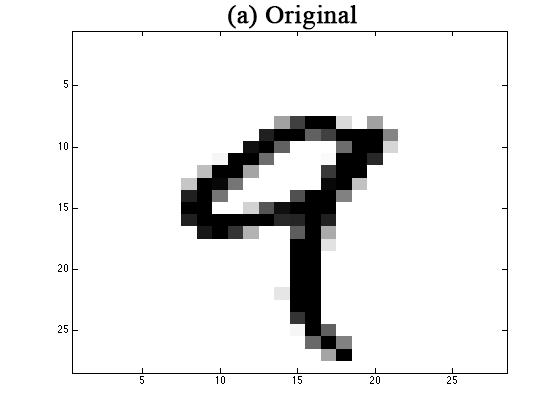
\includegraphics[scale=0.20]{exp/original.png}
 \includegraphics[scale=0.20]{exp/5x5removal.png}
 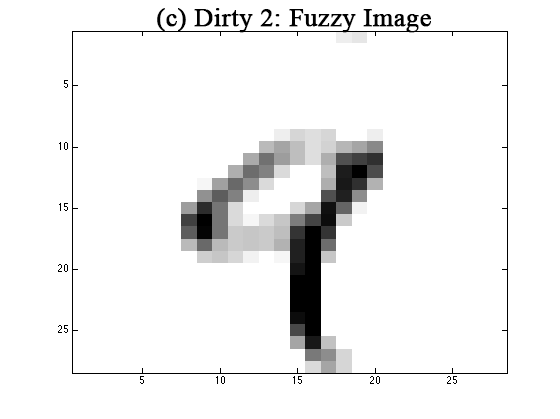
\includegraphics[scale=0.20]{exp/fuzzy.png}
 \caption{We experiment with two forms of corruption in the MNIST image datasets: 5x5 block removal and making the images fuzzy. Image (a) shows an uncorrupted ``9", image (b) shows one corrupted with block removal, and image (c) shows one that is corrupted with fuzziness. \label{mnist-corr}}
\end{figure}